\chapter{Obtención, procesado y almacenamiento de los datos}

Los datos provienen del Gas Drift Dataset del repositorio UCI, 
donde el objetivo era tratar de detectar el drift (la deriva) de los sensores a lo largo de los meses. Están disponibles un total de 13910 mediciones. 

Los datos estan disponibles para su descarga desde
\href{https://archive.ics.uci.edu/ml//datasets/Gas+Sensor+Array+Drift+Dataset#}{UCI data repository}.
en 10 archivos formato \emph{.dat}. Cada archivo .dat contiene una codificación tipo libsvm x:v,
 donde x representa el número de característica y v el valor real de la característica. 
 Por ejemplo, en 1; 10.000000 1: 15596.162100 2: 1.868245 3: 2.371604 4: 2.803678 5: 7.512213 ... 128:-2.654529

X sería 1;10.000, que nos dice que se trata del gas 1 con una concentración de 10, y a continuación las 128 componentes obtenidas de los sensores.
con 129 columnas,
donde la primera nos informa del gas y la concentración, y el resto es la información obtenida del sensor.

\section{Procesado}

La lectura de los archivos \emph{.dat} se ha realizado utilizando una librería que se ha creado para cargar de forma rápida y cómoda todos los datos en un Dataframe de Pandas. El código adjunto en Apéndices \ref{LoadUciData}.

\section{Exploratory Data Analysis}

Los datos se nos presentan en 10 lotes, correspondientes a experimentos a lo largo de tres años, donde se ensayaron 6 diferentes gases a diferentes concentraciones.

\begin{table}[h!]
\begin{tabular}{>{\bfseries}l|l|}
\toprule
Batch ID & Month IDs                   \\ \midrule
Batch 1  & Months 1 and 2              \\
Batch 2  & Months 3, 4, 8, 9 and 10    \\
Batch 3  & Months 11, 12, and 13       \\
Batch 4  & Months 14 and 15            \\
Batch 5  & Month 16                    \\
Batch 6  & Months 17, 18, 19, and 20   \\
Batch 7  & Month 21                    \\
Batch 8  & Months 22 and 23            \\
Batch 9  & Months 24 and 30            \\
Batch 10 & Month 36                    \\ \bottomrule
\end{tabular}
\caption{Distribución de los lotes a lo largo del tiempo. \label{Tab: batch_month}}
\end{table}

Los gases que se estudiaron son los siguientes:
\begin{itemize}
    \item Ethanol
    \item Ethylene
    \item Ammonia
    \item Acetaldehyde
    \item Acetone
    \item Toluene
\end{itemize}

Los lotes contienen una cantidad de muestras desigual, ni los 6 gases de estudio están presentes en todos los lotes. La tabla \ref{Tab: Numero de Gases por cada Batch} muestra el numero de ensayos para cada gas.

\begin{table}
    \centering
    \begin{tabular}{>{\bfseries}l|l|l|l|l|l|l|l|}
    \toprule
        Batch ID & GAS1 & GAS2 & GAS3 & GAS4 & GAS5 & GAS6 \\  \midrule
        1 & 90   & 98  & 83  & 30  & 70  & 74   \\ \hline
        2 & 164  & 334 & 100 & 109 & 532 & 5    \\ \hline
        3 & 365  & 490 & 216 & 240 & 275 & 0    \\ \hline
        4 & 64   & 43  & 12  & 30  & 12  & 0    \\ \hline
        5 & 28   & 40  & 20  & 46  & 63  & 0    \\ \hline
        6 & 514  & 574 & 110 & 29  & 606 & 467  \\ \hline
        7 & 649  & 662 & 360 & 744 & 630 & 568  \\ \hline
        8 & 30   & 30  & 40  & 33  & 143 & 18   \\ \hline
        9 & 61   & 55  & 100 & 75  & 78  & 101  \\ \hline
        10 & 600 & 600 & 600 & 600 & 600 & 600  \\ \bottomrule
    \end{tabular}
    \caption{Numero de gases ensayados por batch. Notar que el gas 6 en los lotes 3,4 y 5 no está presente. \label{Tab: Numero de Gases por cada Batch}}
\end{table}


En la Tabla\ref{Tab: Numero de Gases por cada Batch} podemos ver que el número de muestras en cada lote es desigual. En los lotes 3, 4 y 5 el gas 6 no está presente. A la hora de crear un dataset de entrenamiento,
convendría generar un lote donde haya un numero equitativo de muestras de todos los gases,
y si las mediciones no son distantes en el tiempo podremos ver el efecto de la deriva si el algoritmo entrenado con
los primeros lotes falla para cada vez más conforme nos alejamos en el tiempo.

La Figura \ref{fig: gasBatchCount} muestra la cantidad de gases ensayados por lote, mientras que
la Figura\ref{fig: gasCount} muestra el numero de mediciones totales sobre cada gas.

\begin{figure}[ht!]
	\centering
	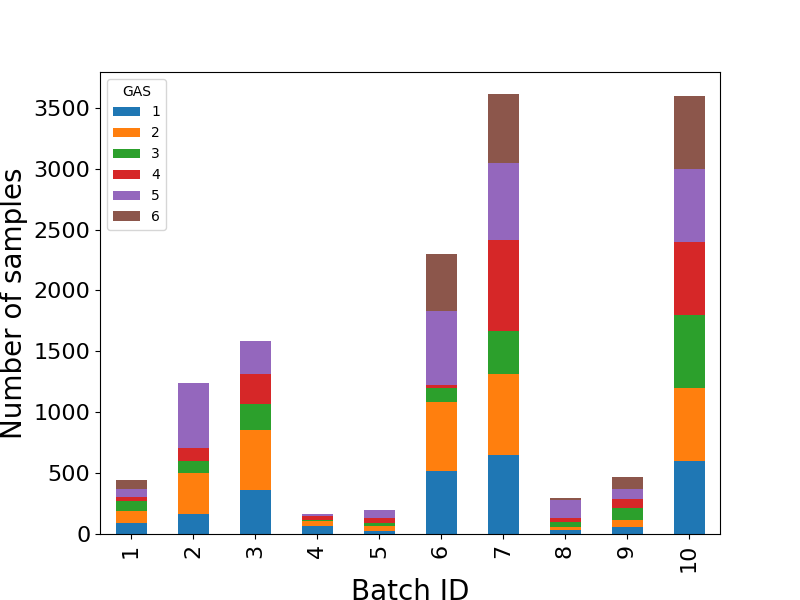
\includegraphics[width=\columnwidth]{../py_imgs/Step0_Count_Batch_Gas.png}
	\caption{Número de muestras de gas por Batch. El número de muestras ensayadas en cada lote es muy desigual, donde los lotes 1,4,5,8 y 9 cuentan con muchas menos mediciones que el resto. }
	\label{fig: gasBatchCount}
\end{figure}

\begin{figure}[ht!]
	\centering
	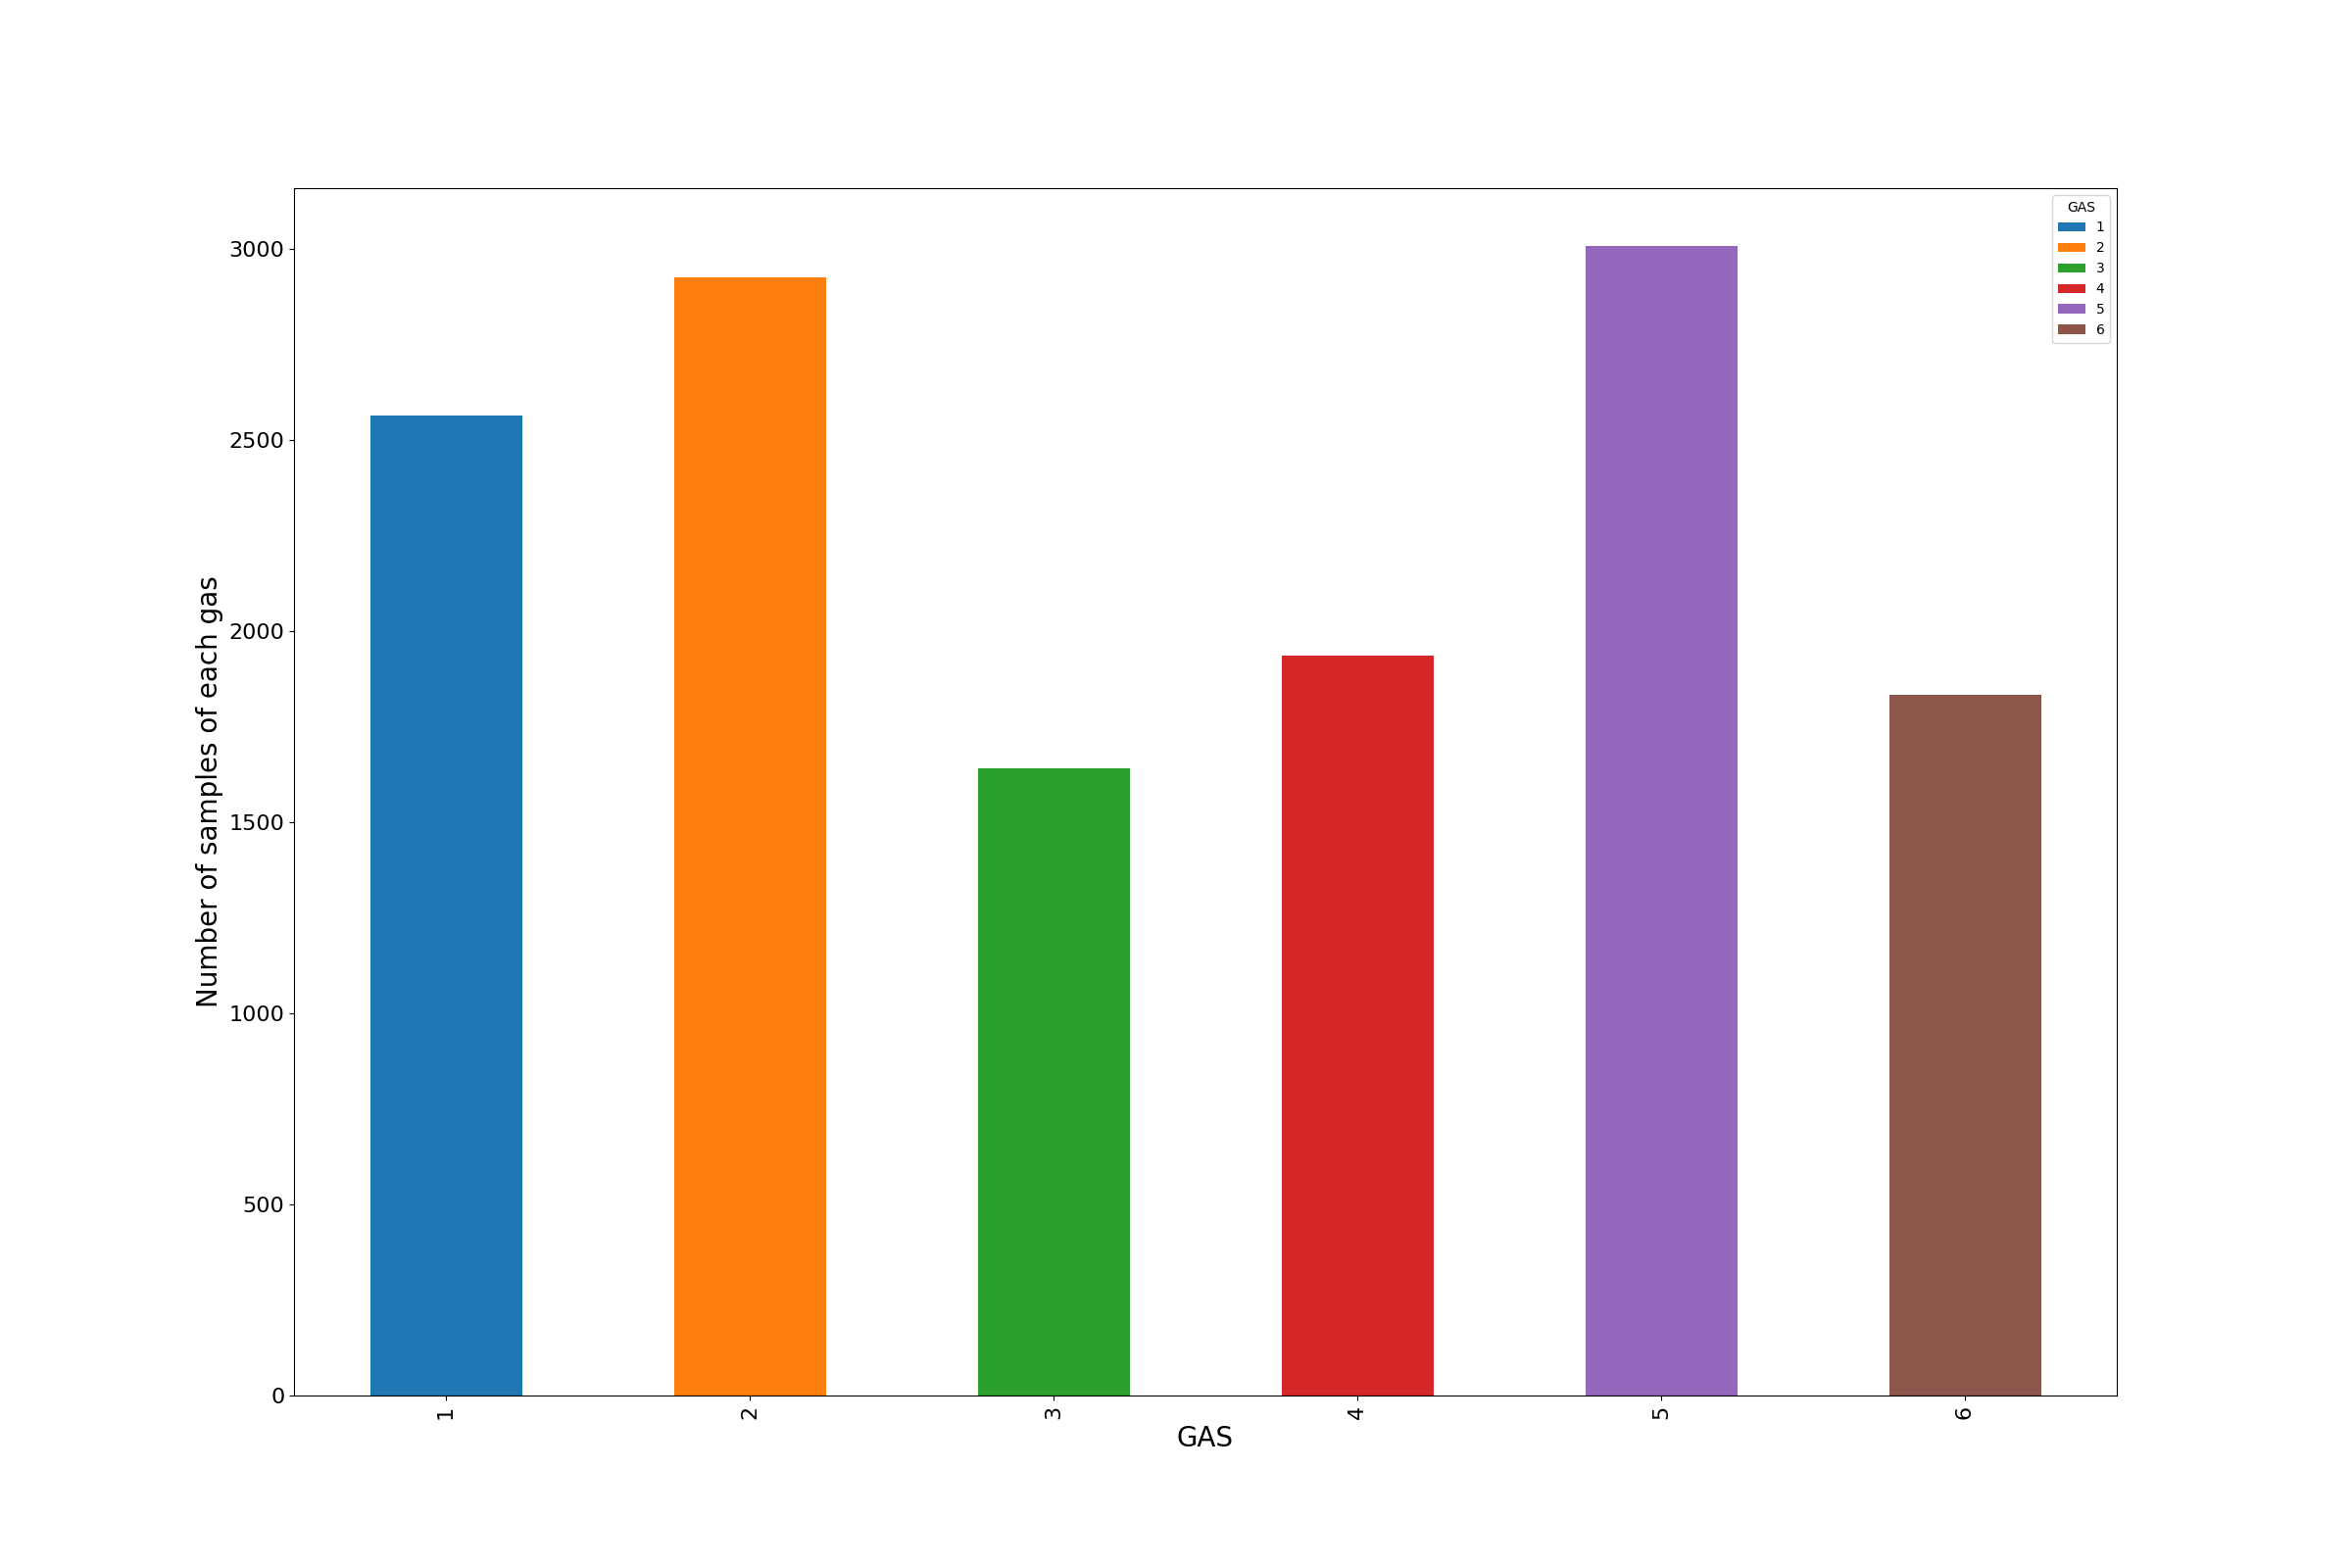
\includegraphics[width=\columnwidth]{../py_imgs/Step0_Count_Gas.png}
	\caption{Número de muestras de cada gas en total}
	\label{fig: gasCount}
\end{figure}

En la Tabla \ref{Tab:Variación de las concentraciones} los rangos de concentración para cada gas, han sido también diferentes.

\begin{table}
    \centering
    \begin{tabular}{|l|l|l|l|l|l|}
    \toprule
    GAS & Minimo & Máximo & Media  & StdDesv \\ \midrule
        1 & 2.5 & 600    & 114.95 & 86.64          \\ \hline
        2 & 2.5 & 300    & 116.1  & 79.89          \\ \hline
        3 & 2.5 & 1000   & 323.55 & 272.02         \\ \hline
        4 & 2.5 & 300    & 126.32 & 76.71          \\ \hline
        5 & 10  & 1000   & 228.57 & 217.38         \\ \hline
        6 & 1   & 230    & 47.66  & 32.58          \\ \bottomrule
    \end{tabular}
	\caption{ Rango de variación de la concentraciones en ppmv utilizadas en las mediciones de los diferentes gases. \label{Tab:Variación de las concentraciones}}
\end{table}

En la Figura\ref{fig:step0concentration-distribution-per-gas} se ha realizado un recuento de cuantas muestra para cada par gas-concentración están disponibles dentro de las 13910 muestras.

\begin{figure}
	\centering
	\includegraphics[width=\linewidth]{"../py_imgs/Step0_Concentration Distribution per gas"}
	\caption{ Recuento del numero de muestras disponibles. El eje de abscisas no es continuo, solo muestra de forma ordenada de menor a mayor las concentraciones disponibles en el dataset. }
	\label{fig:step0concentration-distribution-per-gas}
\end{figure}

\begin{figure}
	\centering
	\includegraphics[width=\linewidth]{"../py_imgs/Step0_Concentration Distribution per gas_binned"}
	\caption{Recuento del numero de muestras disponibles, agrupadas por intervalos. De esta forma es más visual poder apreciar el rango de variación de la concentración para cada gas.}
	\label{fig:step0concentration-distribution-per-gas_binned}
\end{figure}

A la vista de la distribución de concentraciones disponibles, para eliminar el efecto de la concentración en la señal generada por el gas, utilizaremos la concentración más ensayada para cada gas. 

\begin{table}
	\centering
	\begin{tabular}{|l|l|l|}
		\toprule
		GAS & CONCENTRACIÓN & Numero de muestras \\ \midrule
		1   & 50  & 488 \\ \hline
		2   & 50  & 588 \\ \hline
		3   & 200 & 177 \\ \hline
		4   & 100 & 357 \\ \hline
		5   & 50  & 485 \\ \hline
		6   & 50  & 345 \\ \bottomrule
	\end{tabular}
	\caption{Par de gas-concentración qué más mediciones se han realizado. Existen menos muestras disponibles para el par 2-200, pero se trata de suficientes muestras para poder entrenar un modelo.  \label{Tab:Par gas-concentracion habitual}}
\end{table}

\begin{figure}[ht!]
	\centering
	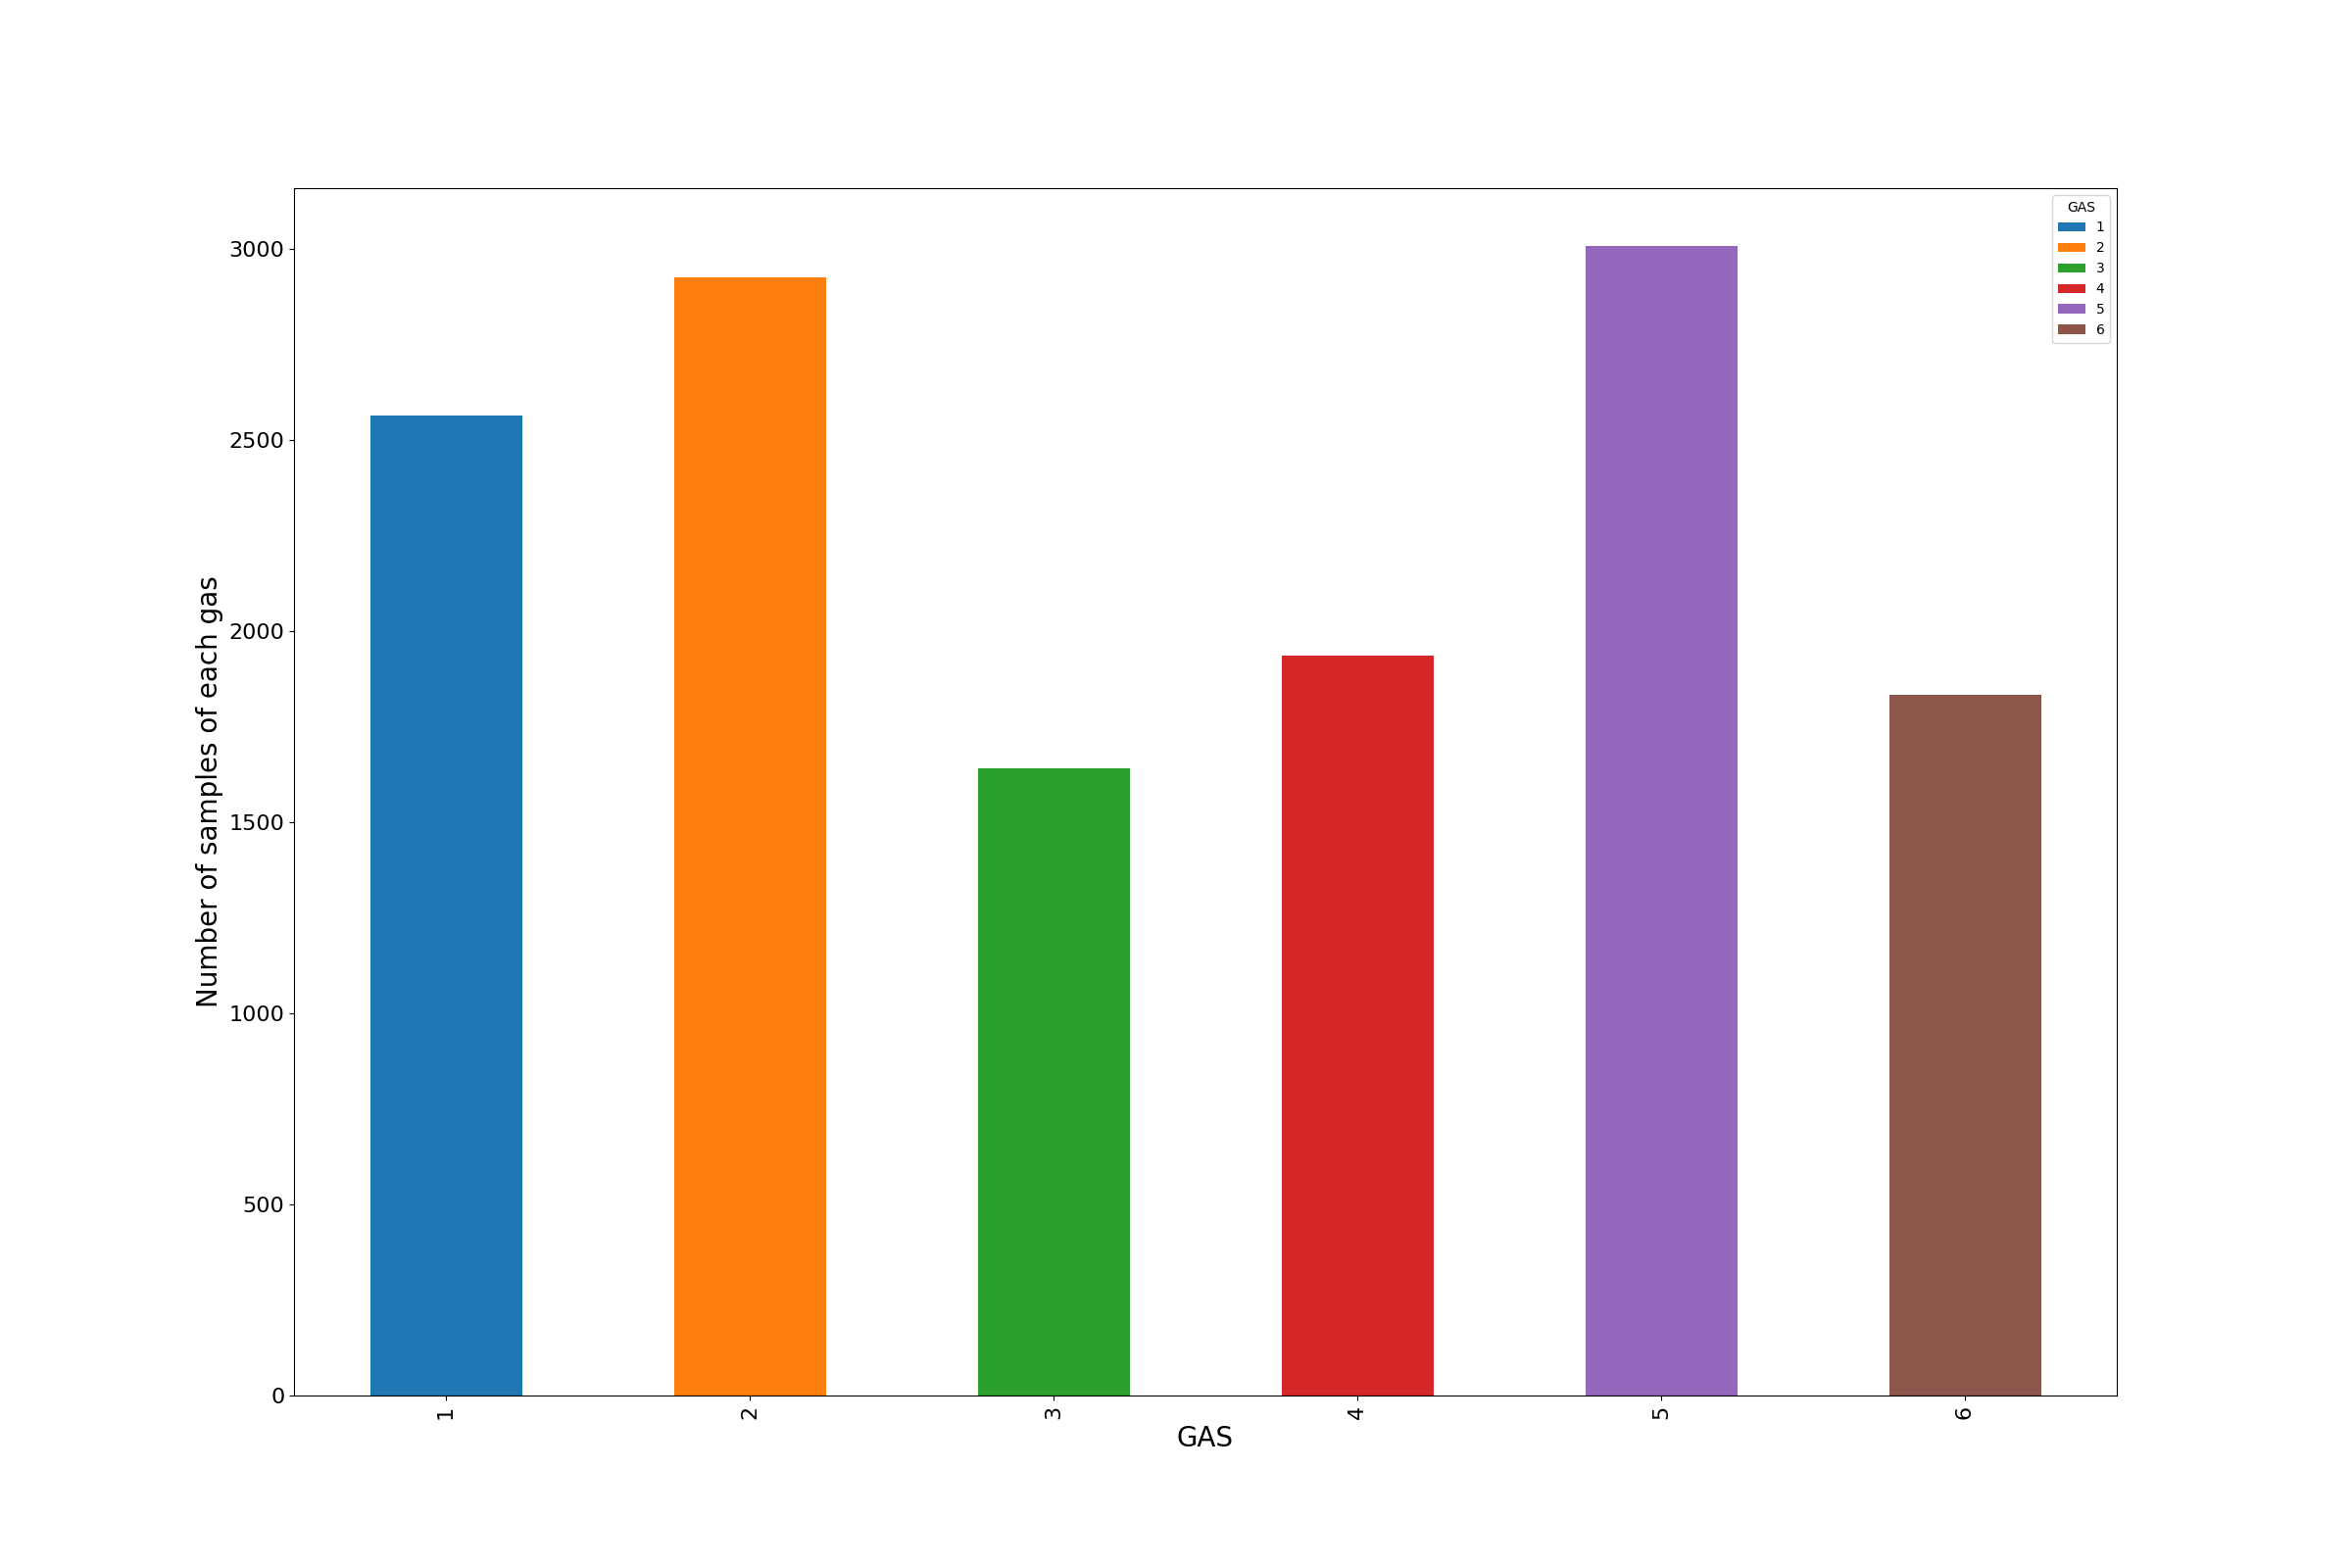
\includegraphics[width=\columnwidth]{../py_imgs/Step0_Count_Gas.png}
	\caption[Número de muestras por gas]{Número de muestras de cada gas en total}
	\label{fig: gasCount}
\end{figure}


Esta información es necesario tenerla en cuenta a la hora de entrenar nuestro modelo, ya que
si el rango de variación de los datos es dispar, será recomendable realizar una normalización de los mismos para evitar perder la información contenida en las variables con un rango menor.


\section{Nota sobre los sensores}

Hay que tener presente que los 16 sensores están generando señales similares y correlacionadas. En la Figura\ref{fig:step01sensorfeaturescolor} queda reflejado cómo las diferencias entre cada sensor/calibración son claras. 

\begin{figure}
	\centering
	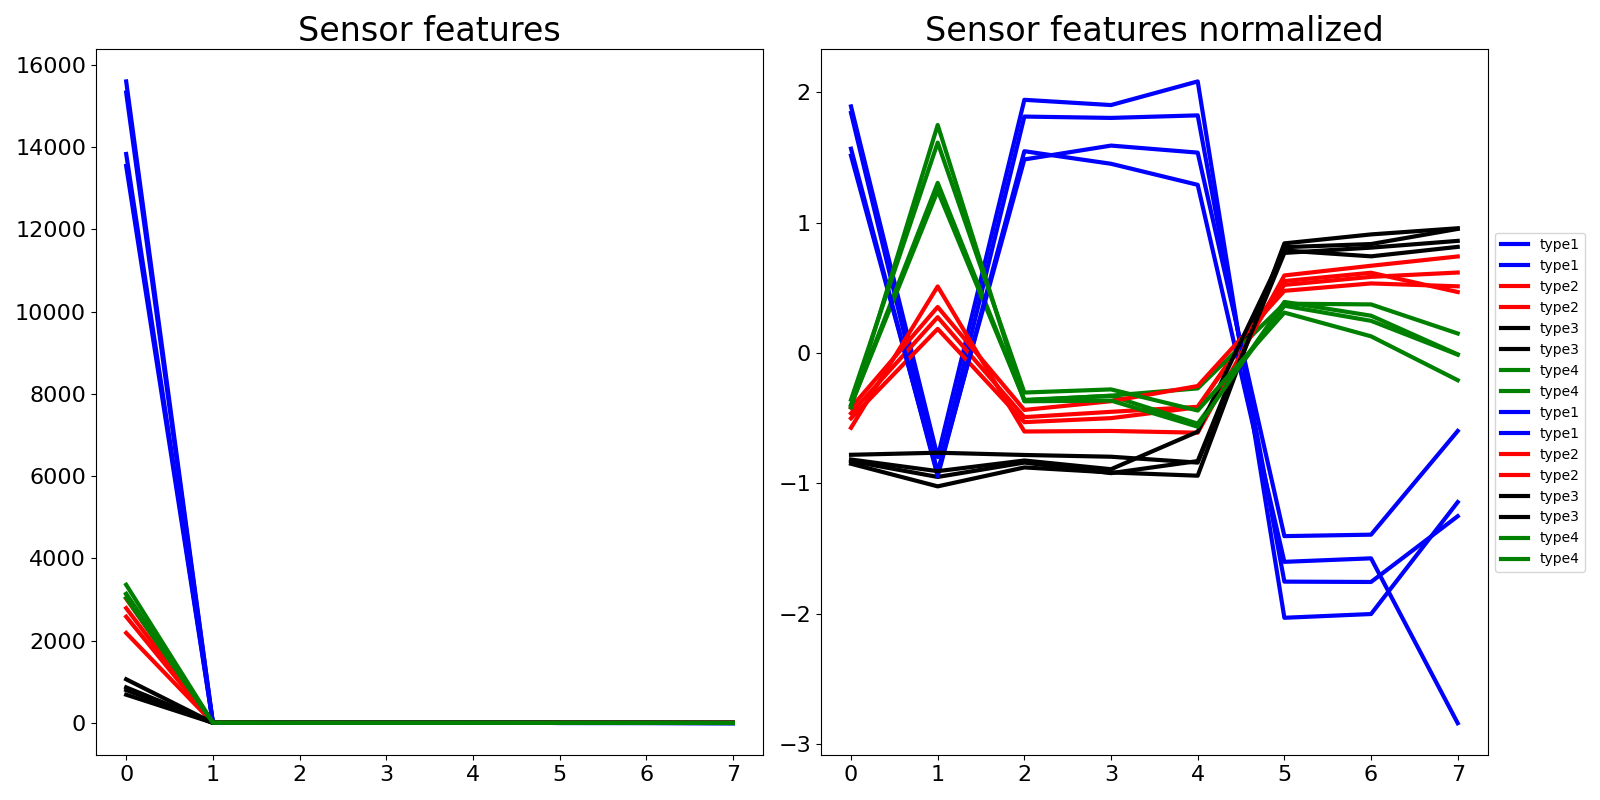
\includegraphics[width=1\linewidth]{../py_imgs/Step0_1_SensorFeaturesColor}
	\caption[Señales de los sensores coloreadas por tipo.]{En el ejeX tenemos las 8 componentes que definen la señal de un sensor. Las señales están coloreadas según el tipo de sensor, al que se le ha denominado Tipo 1,2,3 y 4. A la ize la img muestra las señales tal como están presentes en el dataset, y a la drch están normalizadas. }
	\label{fig:step01sensorfeaturescolor}
\end{figure}

Esto es un problema a la hora de alimentar a los modelos con variables independientes. En la Figura\ref{fig:step011correlationbetweenfeatures} se ha representado el mapa de correlación de las 128 componentes. Para mayor claridad en la Figura\ref{fig:step011correlationbetweenfeaturesdata1} se han representado las features correspondientes a los sensores de diferentes tipos. Puede verse de forma clara cómo existe una correlacion fuerte, tanto positiva como negativa, entre las variables que alimentarán el modelo.

\begin{figure}
	\centering
	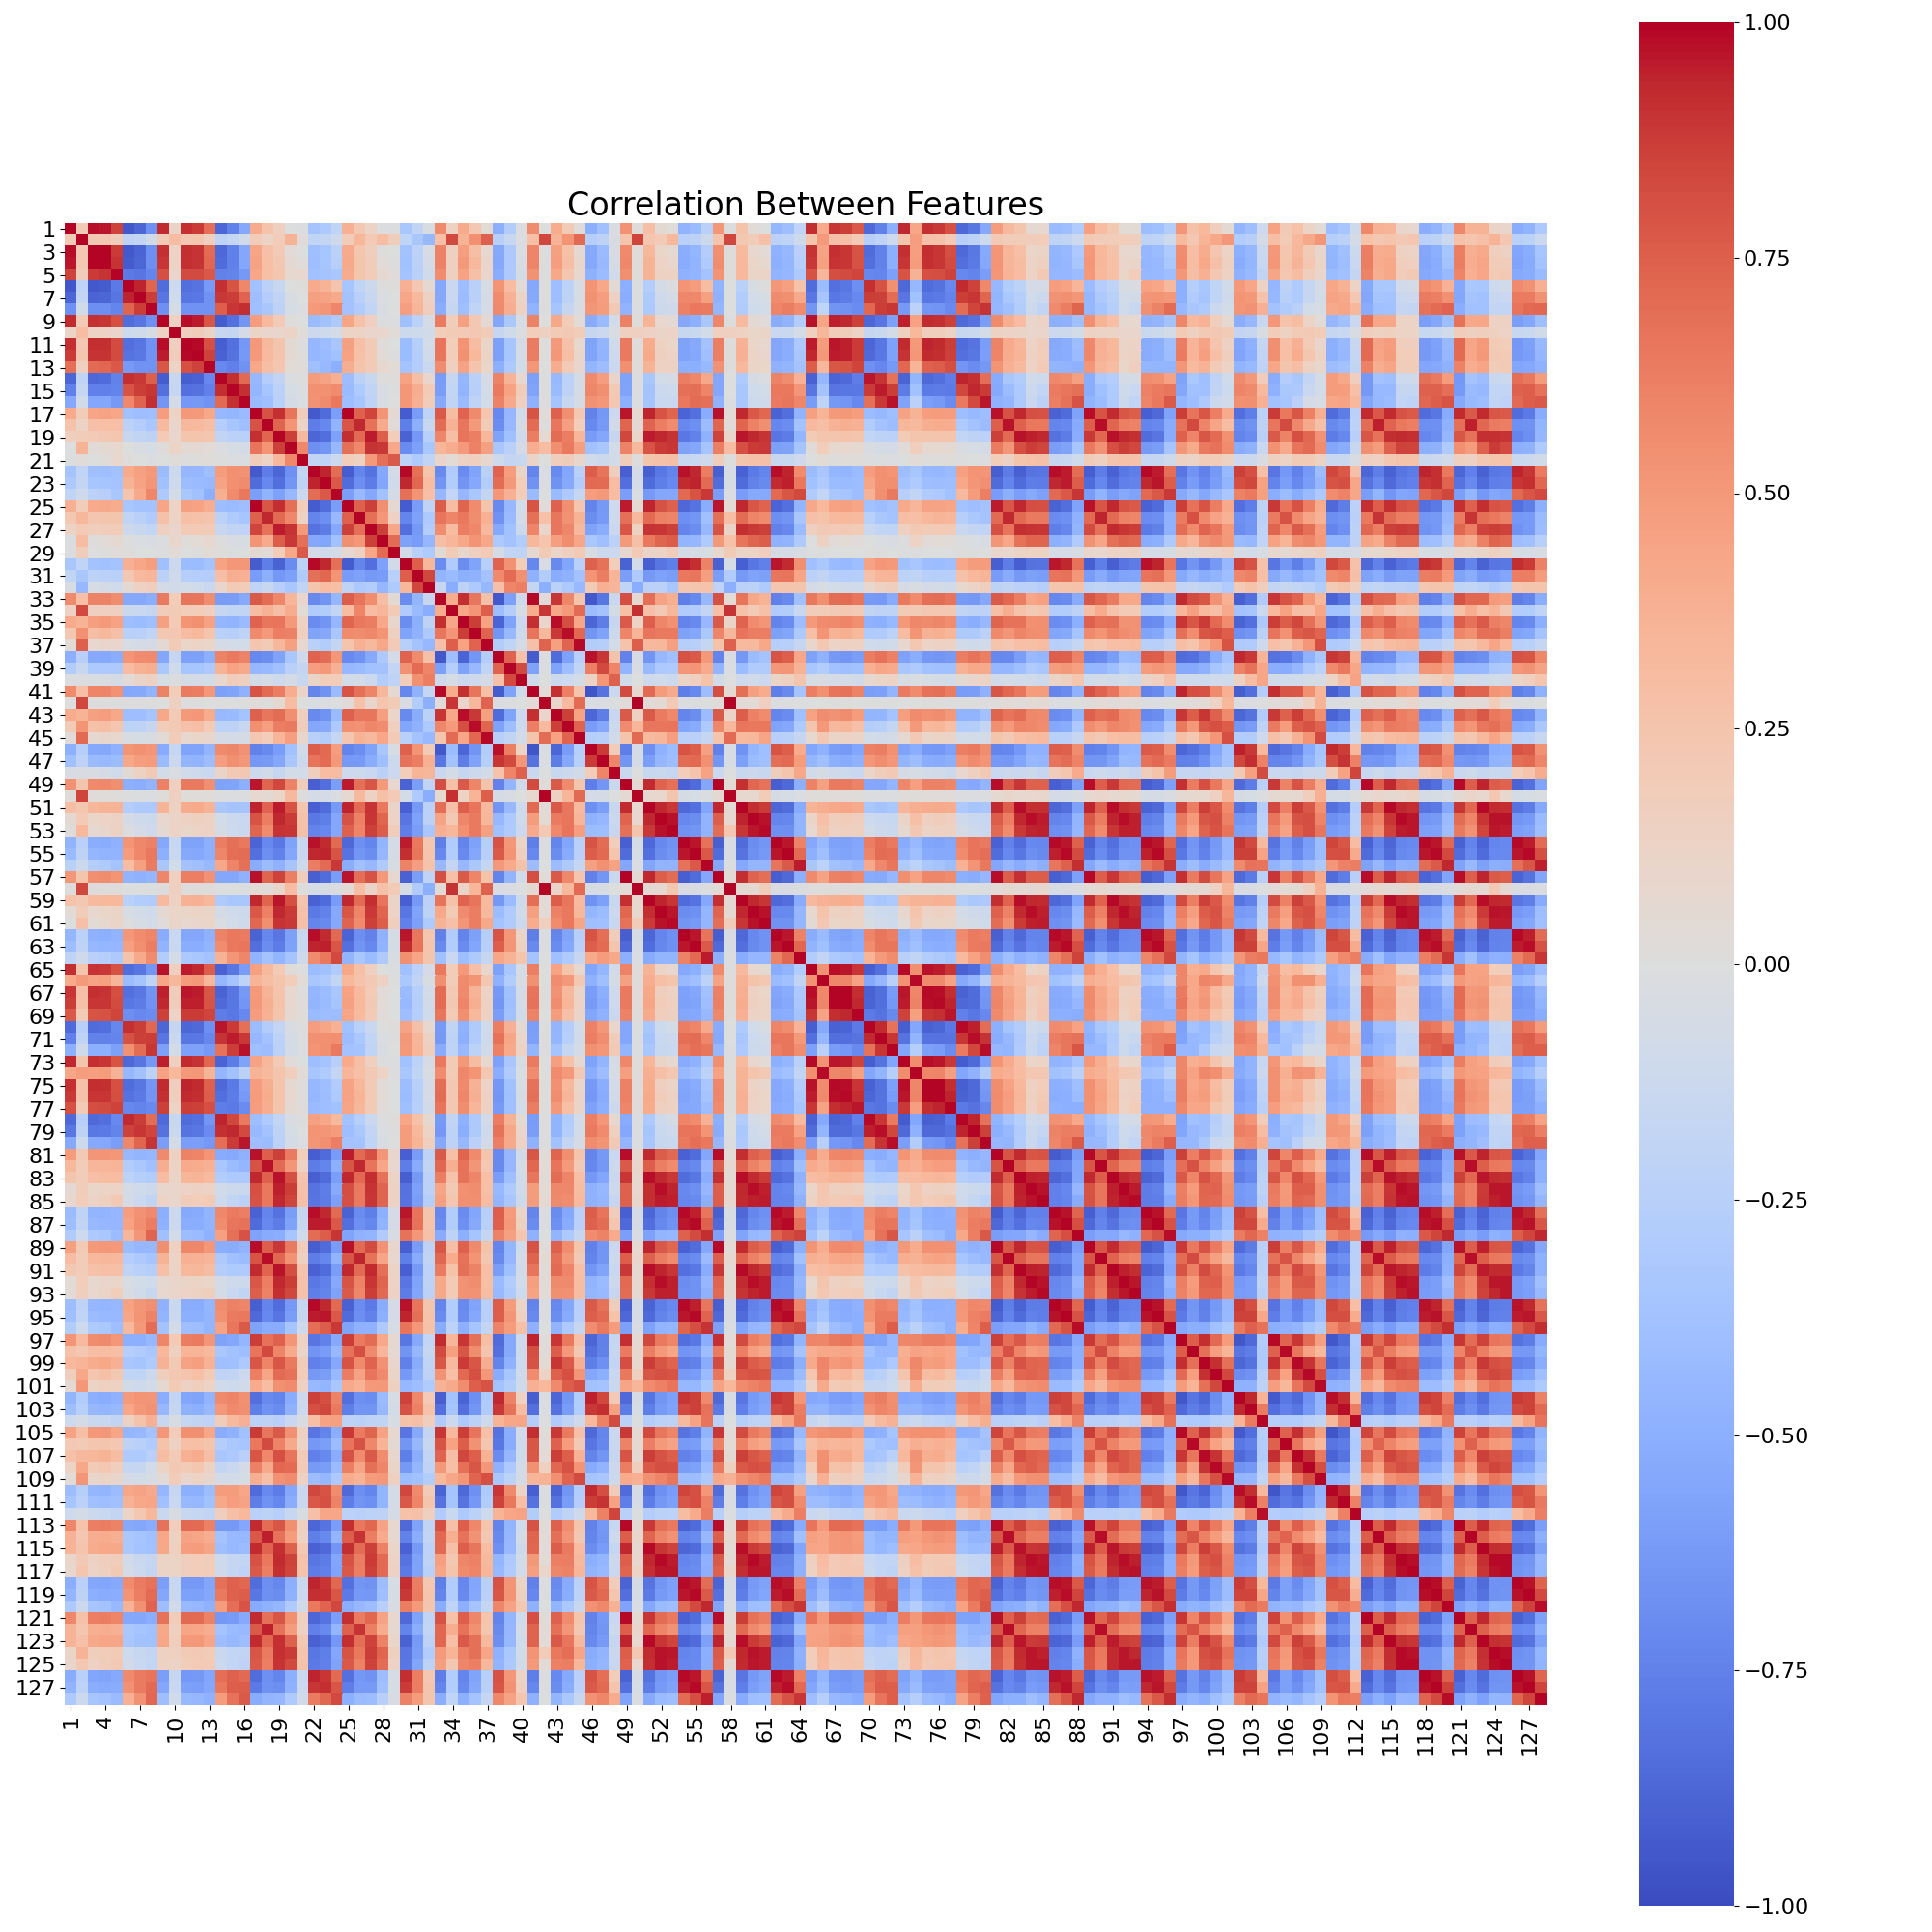
\includegraphics[width=1\linewidth]{../py_imgs/Step0_1_1_CorrelationBetweenFeatures}
	\caption[Correlation map dataset]{Correlación entre las 128 componentes del dataset.}
	\label{fig:step011correlationbetweenfeatures}
\end{figure}

\begin{figure}
	\centering
	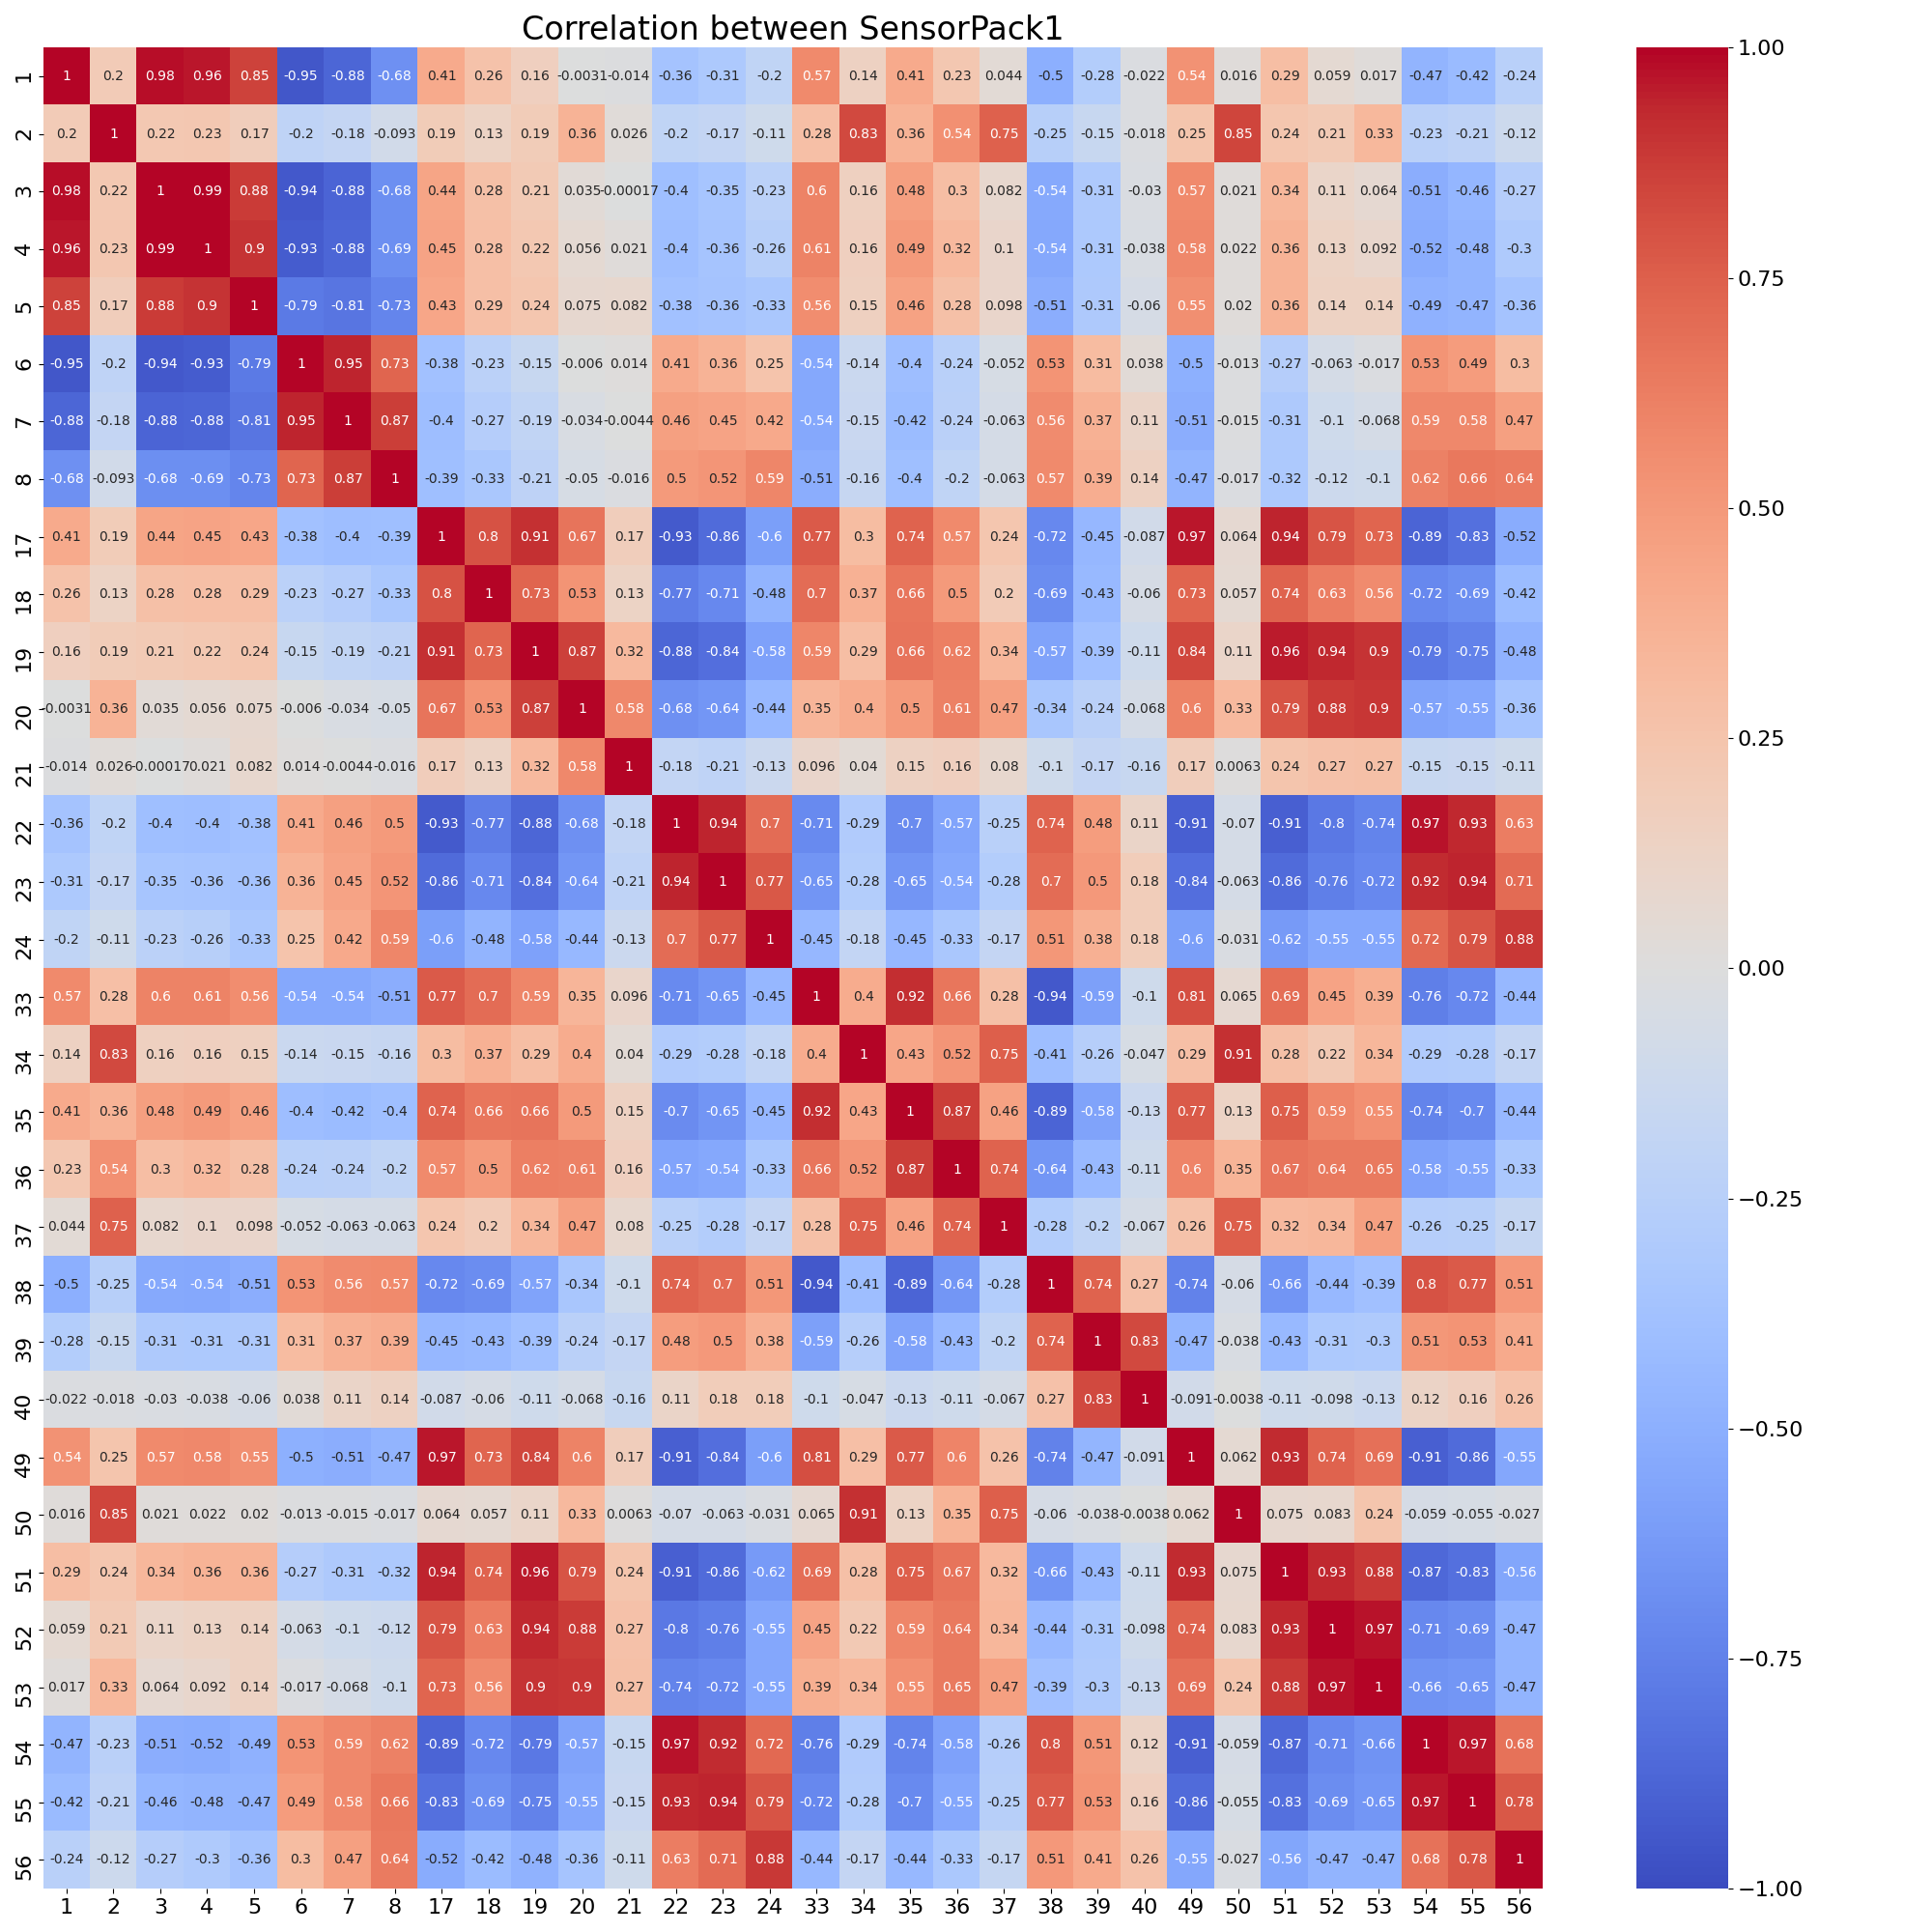
\includegraphics[width=0.7\linewidth]{../py_imgs/Step0_1_1_CorrelationBetweenFeatures_Data1}
	\caption[Correlation map de 4 sensores de cada tipo]{Correlación entre las 128 componentes de 4 sensores de diferentes tipos.}
	\label{fig:step011correlationbetweenfeaturesdata1}
\end{figure}


\section{Evolución  visual del drift}

Se va a proceder a dibujar la señal generada por el sensor 1 de un par gas-concentración, en los diferentes batches, y así ver la deriva de la señal generada. Escogemos para tal tarea el par gas 2 con concentraciones entre 1 y 100.


Dado que las componentes estacionarias y transitorias tienen magnitudes muy diferentes, para ayudar a su visualización realizamos un escalado estándar.

\begin{figure}[h!]
	\centering
	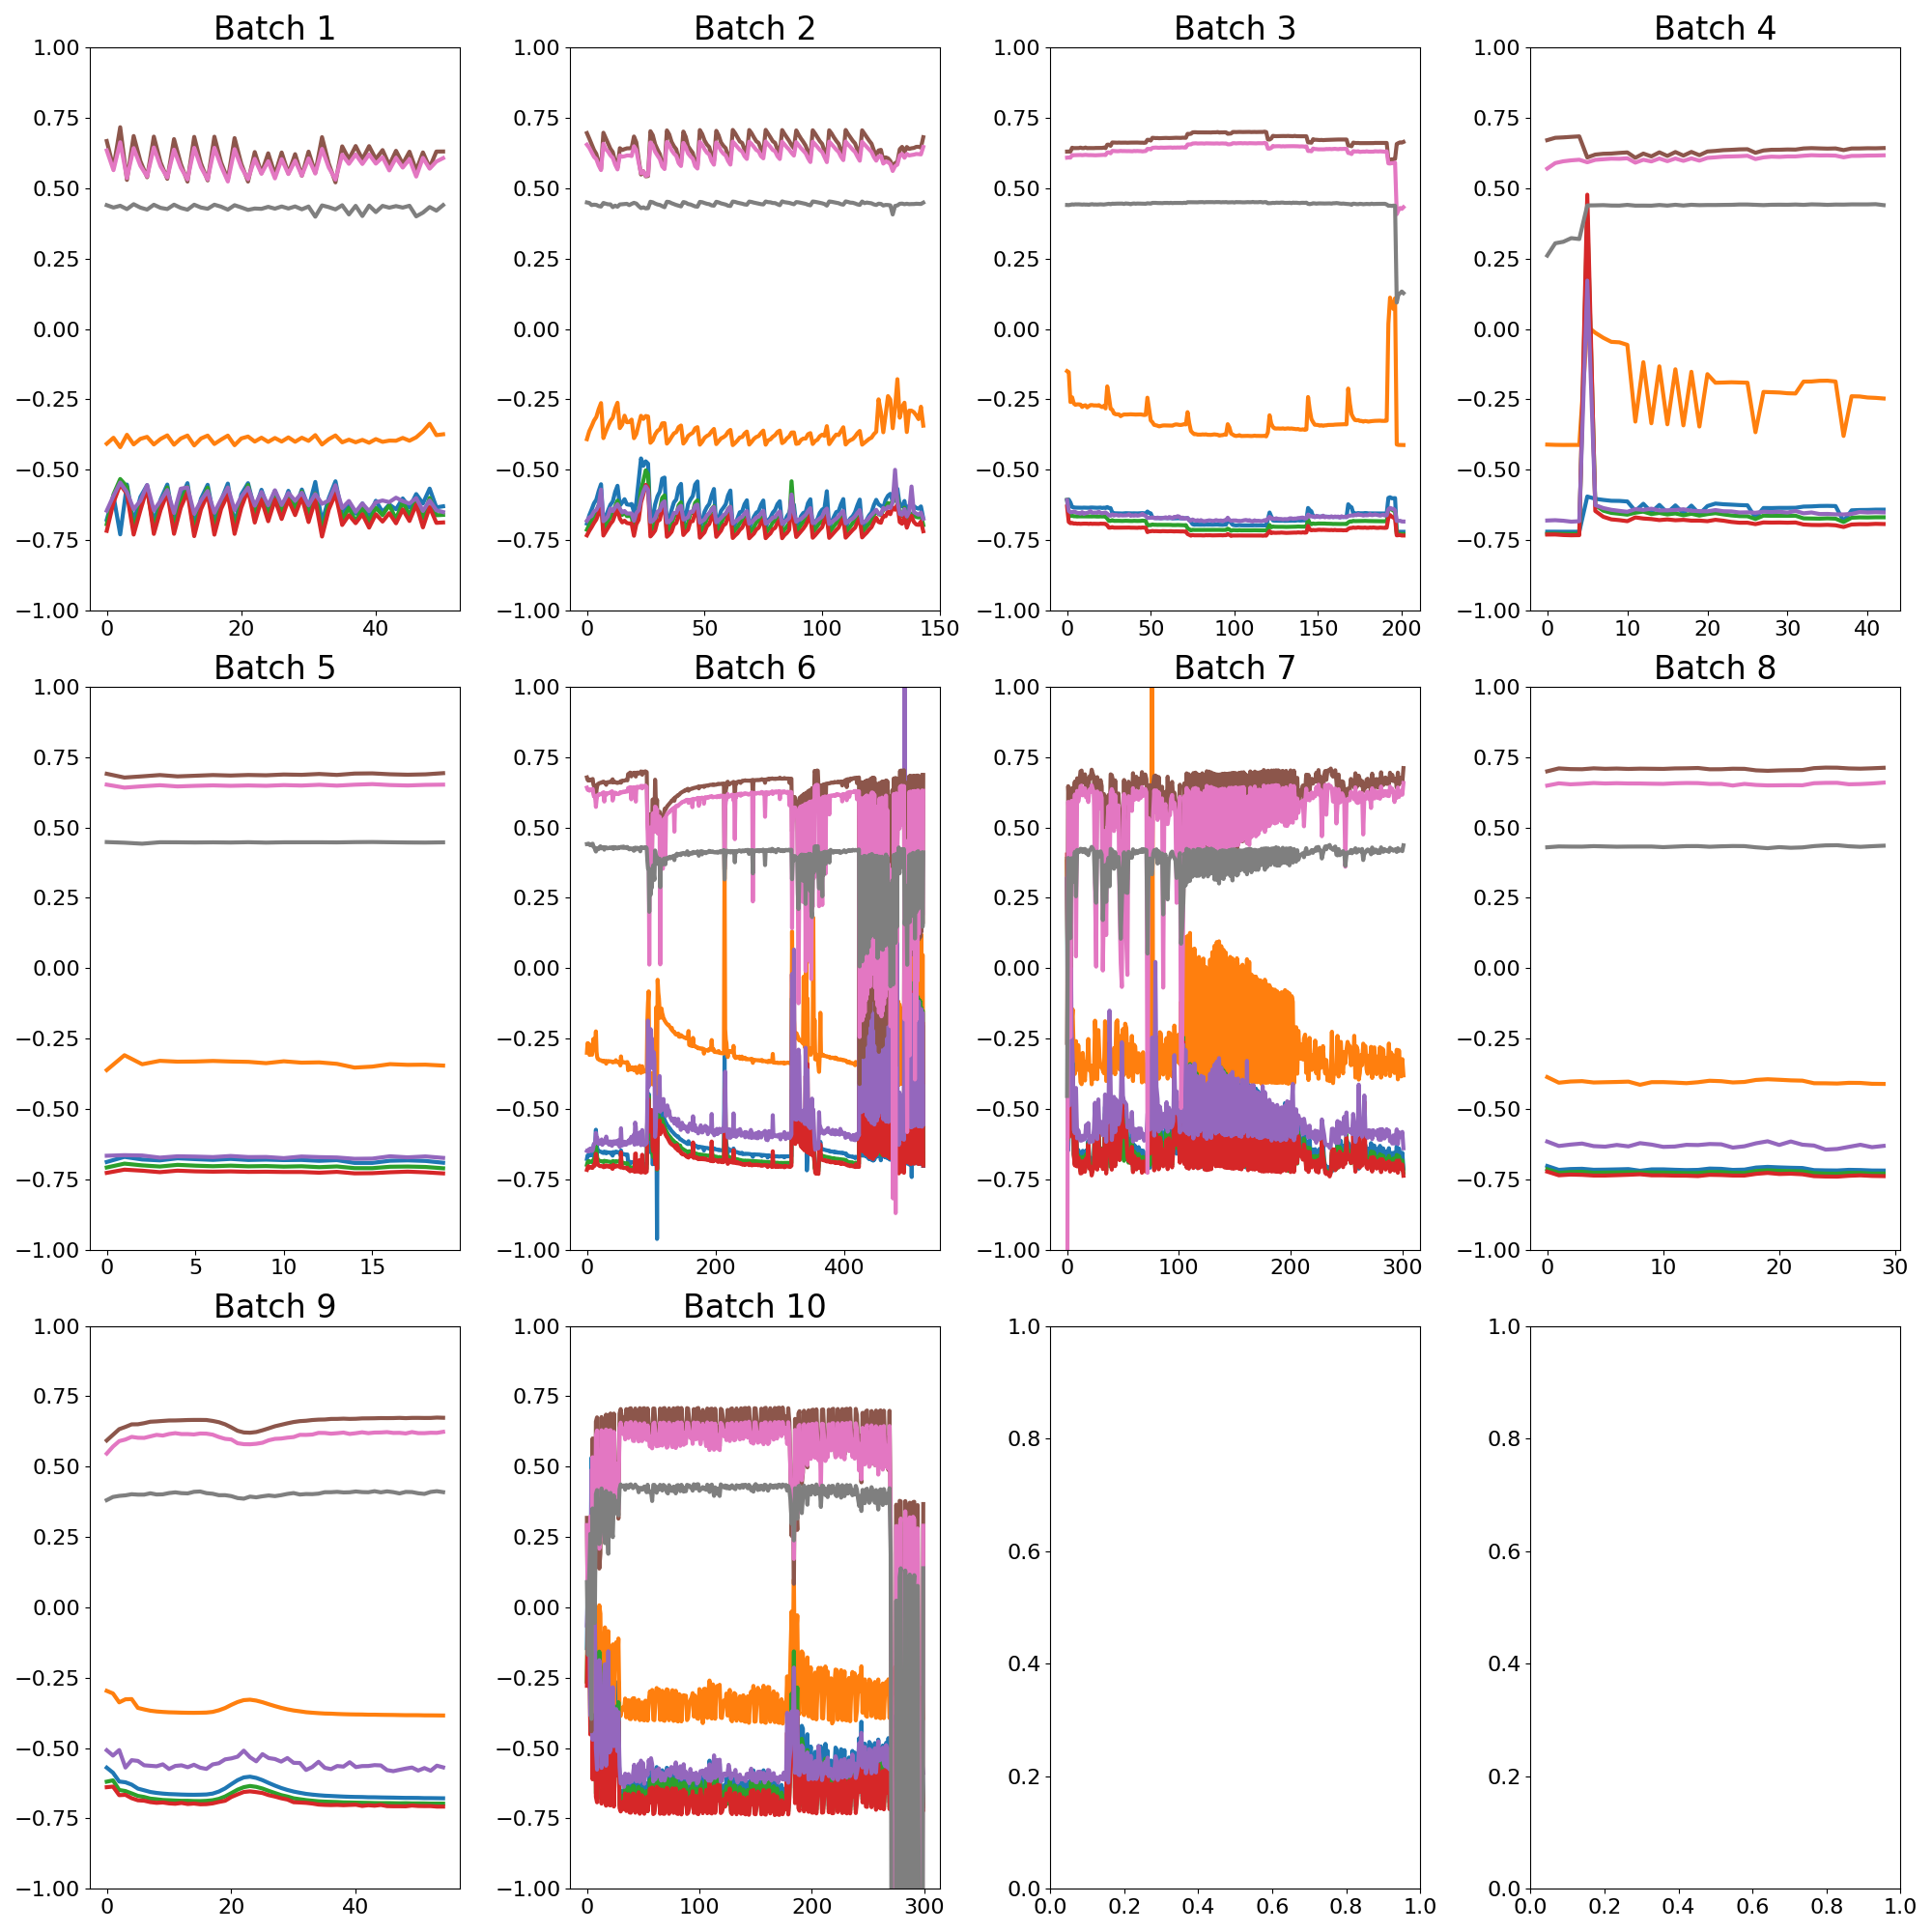
\includegraphics[width=1\linewidth]{../py_imgs/Step0_Evolution_of_signal_sensor1}
	\caption[Señales disponibles para Gas 2, concentraciones 1-100, evolucion para cada batch]{Para cada batch, se han representado todas las señales disponibles para el Gas 2 y concentraciones en el rango de 1 a 100 ppvm. A simple vista no puede apreciarse la deriva del sensor.}
	\label{fig:step0evolutionofsignalsensor1}
\end{figure}

No puede apreciarse a simple vista el efecto de la deriva del sensor. Si realizamos la media de todas las mediciones realizadas en cada batch \ref{fig:step0evolutionofsignalsensor1_mean}, vemos que la firma del gas 2 no cambia de forma visible.

\begin{figure}[h!]
	\centering
	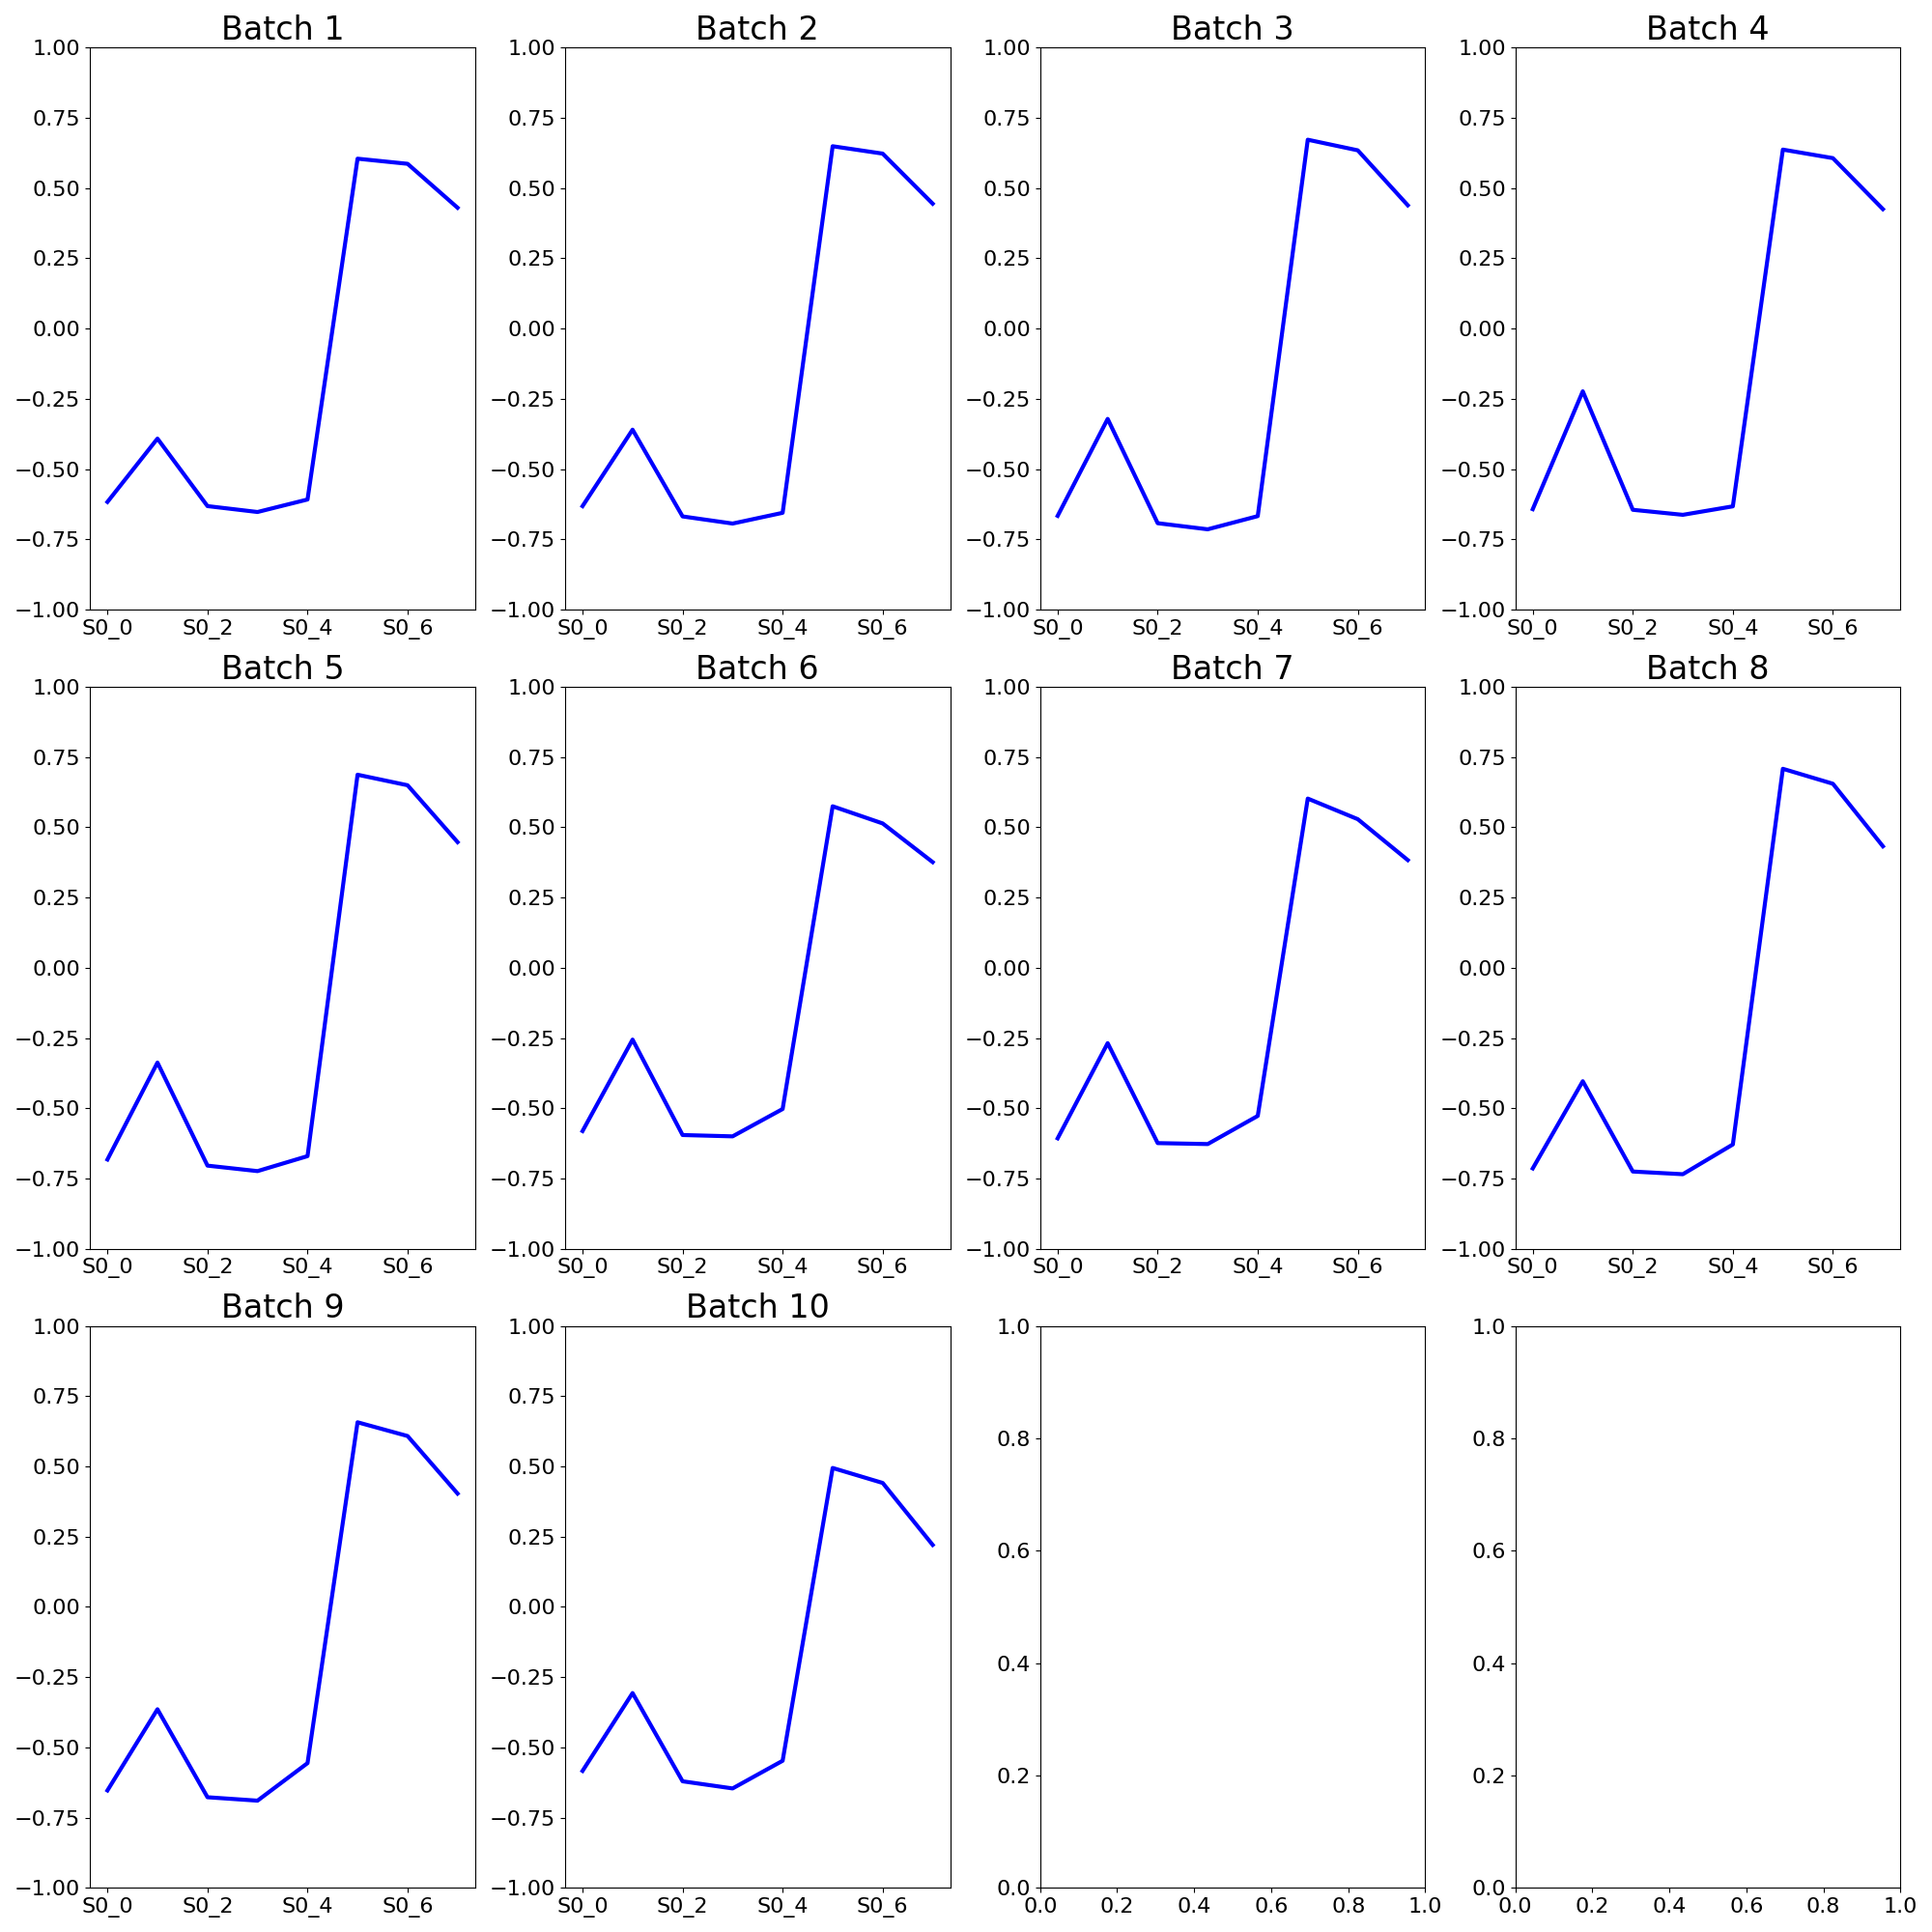
\includegraphics[width=1\linewidth]{../py_imgs/Step0_Evolution_of_signal_sensor1_mean}
	\caption[Media de las señales disponibles para Gas 2, concentraciones 1-100, evolucion para cada batch]{Para cada batch, se ha calculado la media de todas las señales disponibles para el Gas 2 y concentraciones en el rango de 1 a 100 ppvm. En el ejeX, la nomenclatura $SX\_Y$ significa SensorX, featureY, indexado en cero.}
	\label{fig:step0evolutionofsignalsensor1_mean}
\end{figure}




